\section*{Office Duties}
\begin{center}
\uppercase{\Large\underline{\textbf{Overview}}}
\end{center}

\textbf{Duties Include:}
\begin{easylist}[itemize]
& Each work day:
&& Check P.O. Box and office mailbox for payments and invoices.
&& Check phone/email messages, respond to customer requests, page/\\call
operator with repairs.
&& Stamp all incoming mail with date received and sorry accordingly.
& Each week:
&& Input bill payments in RVS system.
&& Prepare deposits and take to bank.
& Each month:
&& Attend board meetings and record/prepare minutes and folders for board members.
&& Prepare and post meeting agendas 72 hours prior to each meeting. (Before 7:00 pm on the Friday before the meeting.)
&& Prepare and mail monthly bills to members by the 10\textsuperscript{th}.
&& Print meter reading worksheets for meter reader in order for him or her to read meters at the end of the month.
& Write correspondence. This includes member transfers, change of address, etc. Any changes that result in changes in the RVS system are to be entered into the system.
& Maintain/Balance petty cash fund in lockbox with receipts of transactions.
& Maintain postage to ensure at least two months worth of stamps (approximately three rolls of post card stamps and one roll of forever stamps used power month) to cover post card and sealed envelope mailings. Notify post office two days before purchase to ensure availability.
& Buy and maintain office supplies.
& Prepare/Maintain office and member files.
\end{easylist}


\newpage
\begin{center}
\uppercase{\Large\underline{\textbf{Daily Duties}}}
\end{center}

The P.O. Box is located at the Weston post office, at 101 Main Street. \textbf{Check the P.O. Box prior your to arrival at the office to ensure the office is staffed during business hours.}

To check the Weston Water email inbox, open a browser and log in to \url{http://gmail.com}\\\textbf{Username:} westonwater@gmail.com\\\textbf{Password:} goatman08

\vspace{1cm}
\begin{center}
\uppercase{\Large\underline{\textbf{Weekly Duties}}}
\end{center}

Find the RVS Mosaics Utility Billing Software on the desktop of the laptop computer and double-click the icon to launch RVS.

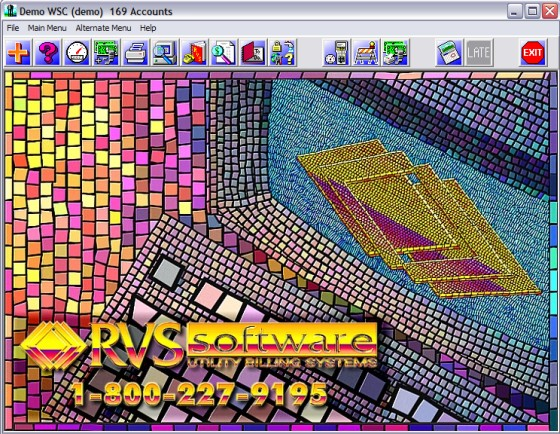
\includegraphics[width=\textwidth]{rvs}

\begin{easylist}[enumerate]
& Add
& Find account by account number or by first 3-4 letters of account holder's last name.
& Enter meter readings.
& Bill
& Print meter reading worksheet.
& Search
& Call RVS
& Search money
& To Do
& Lock
& Meter
& Construction
& Print bill
& Calendar
& Late
& Exit
\end{easylist}

\vspace{1cm}
\begin{center}
\uppercase{\Large\underline{\textbf{Monthly Duties}}}
\end{center}

Post copies of the meeting agenda both in front of the office and in the post office. % and online?